\section{Introduction}
From a designer's perspective, colors play an essential role in cartography. Especially the ability to distinguish colors and shades of the same color can be challenging. In this context, the color distance can be an important factor for the readability of the map. Even discrete manipulations of color spacing show significant effects on the overall readability of a map \parencite{brychtovaC2015,brychtova2015, brychtovaV2014,brychtovaC2016}. Yet, according to \textcite{brychtovaC2017}, there is little research to empirically determine the minimum effective color distance to safely and correctly distinguish cartographic symbols. 

Furthermore, the lack of adequate visual spacing in the hue and chromaticity variables may pose a readability problem in map use \parencite{chesneau2007, steinrucken2013, stigmar2010}.

In this paper, we hypothesize that the differentiability of colors when viewing choropleth maps depends primarily on the color distance between colors and the number of color classes. To do this, we first address a basic understanding of choropleth maps. Then, under the chapter Basic Color Information, we will look at Humans' Color Perception and some Color Models. Furthermore, this work contains the crucial criterion Color Distance, according to which it is easier for the viewer of a map to distinguish colors from each other. In the following chapter, we will look at other aspects that could play a role in this process. In the fourth chapter, we will present two example tools that take color distance into account when creating color schemes. Finally, we summarize the main points and come to a conclusion and a small outlook. 

\subsection{Simple Choropleth Maps}
Unlike chorochromatic maps, which visualize nominal (qualitative) data, simple choropleth maps have made it their business to display quantitative data in terms of area. In doing so, hue, saturation and brightness are used to show corresponding changes in the data. Although in theory choropleth maps are only useful for data related to areas \parencite{hruby2016, schiewe2015}, in practice they are also used for non-area related data e.g. incidence values.

Some advantages of choropleth maps are e.g. the simplified visibility. For this, the data are classified. For example, one can distinguish between an equal interval and a quantile class division. With equal interval each class possesses the same size independently of its occupation, whereas with a quantile class division each class contains the same number of elements. Depending on the use case and data frequency, one or the other class division is more suitable, because they have a significant influence on the appearance of a map \parencite{schiewe2015, rahlf2020}.

Due to the public availability of static data, the production of these maps is easy and can be linked, analyzed, classified and visualized with any suitable GIS software \parencite{hruby2016}.

\section{Basic Color Information}

To understand the following chapters, it is important to know some basics about human color perception and color models.

\subsection{Humans' Color Perception}
Although our current understanding is that color vision results from the response of three photoreceptor cells in the retina to incident light, their perception cannot be fully understood. This may be due to both individual and environmental factors that influence color perception \parencite{lafer2015, xiao2016}.

Some of these factors can be, for example, the amount of light in the environment, shadows, surrounding materials, and reflectivity. In addition, the viewer's prior knowledge and cognitive biases play a significant role in color perception \parencite{derefeldt2004, foster2011}.

In addition, there is evidence that the number and distribution of photoreceptors in the eye influences what we see \textcite{roy1991}, and that our brain assumes a particular direction or light source e.g. \textcite{gegenfurtner2015, lafer2015}.

Thus, it can be said that the color perception of an individual is not stable over space and time. The same is true not only for individuals but also for groups.  

Nevertheless, there are many efforts to model and quantify color perception such as mathematical models that attempt to determine thresholds by which two colors or shades of the same color become distinguishable. 

This color distance describes a metric that quantifies the human ability to visually distinguish differences between two colors see chapter \ref{subsection:distance} \parencite{coltekin2017}.

\subsection{Color Models}
There are a lot of color models that have set themselves the task of representing the logic of generating colors \parencite{kuehni2001}. These color models can be divided into four main groups: instrumental, pseudo-perceptual, colorimetric, and perceptual unitary color models.

In the majority of times we define colors by three RGB values which define the amount of red, green and blue color which combined forms a unique color. Such a color models are called Instrumental color models another example would be the CYMK Model which is used by printers.
Pseudoperceptual color models are e.g. HVS or HSB, whereas colorimetric color models are represented e.g. by CIE 1931 XYZ.
To the latter model (perceptually uniform) belong for example the Munsell system, CIELAB or CIELUV. Such color models tries to make a color model on how human eyes percept the colors. This will be important when calculating a distance between colors how humans see the colors. When calculating the color distance all color modells will play its role except the pseudoreceptual color models. 

A color space is understood to be all existing colors that can be represented e.g. by a screen, printer or the human eye, which are generated from a combination of the components of a model \parencite{munsell1915}. Color spaces are also important cause it is important to know that mediums are limited in the colors they can visualize. When creating a map it should be the goal that the colors used can be visualized by the medium where the map will be shown.  

\section{Criteria}
The following chapter presents criteria that relate to how people distinguish colors on a choropleth map. This is mainly influenced by color spacing, although there are other aspects that can cause difficulties when reading the colors on a map.

\subsection{Color Distance}\label{subsection:distance}
Visual distance in cartography is understood as a measurement of differences between visual variables such as size, shape and orientation \parencite{brychtova2015}. Here we focus on the variable of color hue and color value. The human perceived difference between two colors or color shades can be described as the color distance. In other words, certain change of colour in the perceptually uniform space produces equal change in human perception of that colour \parencite{brychtovaC2017}.

To describe the distance of two colors scientistis have developed a method to describe the color distance. To express color quantitatively a colour space corresponding to the human perception is needed. Such color spaces are called perceptually uniform or linear. The use of such color spaces try to ensure results of color distance which are proportional to the human perception \parencite{brychtova2015}. Presently the CIEDE2000 model ($\Delta E_{00}$, equation defined in \textcite{brychtova2015}) is regarded as the best coinciding color distance model with visual perception. 
 
The colors of digital maps are usually represented in the RGB color space, since the colors on most, if not all, digital screens are generated with these three colors (red, green, blue). However RGB values do not lead to specific color if they are not related to an absolut color space such as sRGB, Adobe RGB or ProPhoto RGB. To use the most realistic color space, colors should be specified and selected in the sRGB color space in the initial situation. Why most realistic? As mentioned before sRGB is the smallest color space of the three. The vast majority of digital screens cannot create all Adobe RGB or even ProPhoto RGB colors. Even sRGB isn't fully supported by cheap laptop screens. However sRGB is known as the default color space \parencite{kenrockwell2006}. Therefore sRGB should be choosed to increase the chance that the users screen actually is able to display the color which was choosed by the creater of a map. 

As a result \textcite{brychtovaC2015, brychtovaC2016} figured out that a color distance of 10 can be considered as a safe color distance.

\subsubsection{Equation}\label{subsec:equation}
The first step to calculate the color distance $\Delta E_{00}$ is the transformation from the original color space (as mentioned above this would be sRGB in most cases) to the CIE 1931 XYZ color space (see equations \ref{equ_1} and \ref{equ_2}). For that the RGB values have to be normalized so the values lie in the interval [0; 1]. 
\begin{equation}\label{equ_1}
R_{lin} = G_{lin} = B_{lin} =
	\begin{cases}
		\frac{V_{R,G,B}}{12.92}, & \text{if $V_{R,G,B} \leq 0.04045$}\\
		\sqrt[5]{(\frac{R + 0.055}{1 + 0.055})^{12}}, & \text{otherwise}
	\end{cases}
\end{equation}
\begin{equation}\label{equ_2}
\left[ \begin{array}{r}
X \\ 
Y \\
Z \\ 
\end{array}\right] = \left[ \begin{array}{rrr}
0.4124 & 0.3576 & 0.1805 \\ 
0.2126 & 0.7152 & 0.0722 \\
0.0193 & 0.1192 & 0.9505 \\ 
\end{array}\right] \left[ \begin{array}{r}
R_{lin} \\ 
G_{lin} \\
B_{lin} \\ 
\end{array}\right]
\end{equation}

The second step is the transformation of the colors into CIE Lab (see  equations \ref{equ_3} - \ref{equ_6}). The CIELAB Colorspace, also known as CIE 1976 (L*, a*, b*) describes all colors perceptible by human eyes \parencite{levkowitz1997}. It consists of three components: L describes the brightness [0 - 100], a describes the axis between red and green and b describes the axis of the blue and yellow colors. While negative values stand for green/blue colors and positive values for magenta and yellow). Theoretically the a and b values are not limited but in praxis human eyes can only see colors upin a specific value. 

\begin{equation}\label{equ_3}
L = 116 f\left(\frac{Y}{Y_{n}}\right)-16
\end{equation}
\begin{equation}\label{equ_4}
a = 500 \left[f\left(\frac{X}{X_{n}}\right)-f\left(\frac{Y}{Y_n}\right)\right]
\end{equation}
\begin{equation}\label{equ_5}
b = 200 \left[f\left(\frac{Y}{Y_{n}}\right)-f\left(\frac{Z}{Z_n}\right)\right]
\end{equation}
where
\begin{equation}\label{equ_6}
f(t) =
\begin{cases}
	\sqrt[3]{t}, & \text{if $t > (\frac{6}{29})^{3}$}\\
	\frac{1}{3}(\frac{29}{6})^{3}t+\frac{4}{29}, & \text{otherwise}
\end{cases}
\end{equation}

Finally the last step is to calculate the color distance $\Delta E_{00}$ between two colors with the CIEDE2000 model (see equation \ref{equ_7}).

\begin{equation}\label{equ_7}
\Delta E_{00}= \sqrt{\left(\frac{\Delta L'}{k_{L}S_{L}}\right)^{2}+\left(\frac{\Delta C'}{k_{C}S_{C}}\right)^{2}+\left(\frac{\Delta H'}{k_{H}S_{H}}\right)^{2}+R_{T}\frac{\Delta C'}{k_{C}S_{C}}\frac{\Delta H'}{k_{H}S_{H}}}
\end{equation}

where $\Delta L'$, $\Delta C'$ and $\Delta H'$ are the CIELAB metric lightness, chroma, and hue differences, calculated
between the standard and sample in a pair and $S_{L}$, $S_{C}$ and $S_{H}$ are the weighting functions for the lightness,
chroma, and hue components.  However, since the formulas are quite extensive, the equations can be read in the appendix \ref{further equation}.
The $k_{L}$, $k_{C}$ and $k_{H}$ values are the parametric factors to be adjusted according to different viewing parameters such as textures, backgrounds, separations etc. \parencite{luo2001}.

\subsection{Further Aspects}
While color distance obviously has the greatest impact on the human ability to distinguish colors, there are several other aspects that play a role. 

\subsubsection{Number of Classes}

Obviously the number of classes also has an impact on the differentiability of colors. For example if we reduce the number of classes to 1 (which makes no sense in practice) the color will be determined in hopefully all cases. The more classes we create, the harder it becomes to tell the colors apart as the propability decreases. In addition to that it is clear that the color distance decreases with more classes as the number of color shades are limited by the color space. 

\textcite{brychtovaC2017} makes the finding that with ColorBrewer 2.0 the color distance becomes smaller the more classes are used, which is to be expected. For the selected 18 sequential schemes, the color distance was analyzed and calculated between 3, 6 and 9 classes. These numbers of classes were selected according to \textcite{brychtovaC2017}, since they represent the minimum, maximum and middle of the class selection. Thus, the results (see table \ref{tab:classes}) show that the number of classes have an influence on how the distance of the colors is chosen and thus becomes distinguishable to the human eye. 

\begin{table}[h!]
\centering
\caption[Color distance depending on number of classes]{Color distance depending on number of classes \\ (According to \textcite{brychtovaC2017})}
	\begin{tabular}{c c c c }
		\hline
		\hline
		Number of classes & $\Delta E_{00}min$ & $\Delta E_{00}max$ & $\Delta E_{00}mean$ \\ 
		\hline
		\hline
		3 & 11.26 & 33.92 & 20.61 \\  
		6 & 6.24 & 26.44 & 12.41 \\
		9 & 3.04 & 20.46 & 10.28   
	\end{tabular}
\label{tab:classes}
\end{table}

\subsubsection{Spatial distance}
The greater the spatial distance between two color cells, the more the ability to distinguish the colors decreases. Especially when the colours are separated by a spatial distance larger than 6�  of visual  angle the difficulty increases. This is true for both sequential and qualitative schemes. However, at a color distance of $\Delta E_{00}$ = 10, the accuracy of color discrimination increases, even at relatively large spatial distances \parencite{article}. 

\subsubsection{Brightness of Colors}

An evaluting case study of color distances in ColorBrewer 2.0 from \textcite{brychtovaC2017} has investigated the color distances in 18 color schemes made by colorBrewer 2.0. All color chemes were investigated with 9, 6 and 3 classes. As a result \textcite{brychtovaC2017} figured out that mostly the darker the color becomes, the larger the color distance becomes (see figure \ref{fig:colordist}). The figure shows the color distance between the colors of six selected color schemes. It can be said that the color distances varies from 5 up to 20.

\begin{figure}[h!]
	\centering
	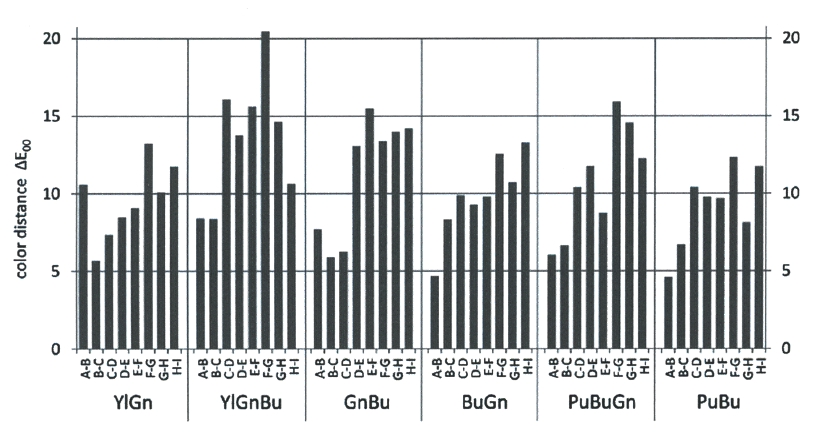
\includegraphics[width=0.7\linewidth]{source/images/colordist}
	\caption{Different schemes with the color distances between their colors. \\
		(Source: \textcite{brychtovaC2017})}
	\label{fig:colordist}
\end{figure}

Therefore it can be assumed that the deveolpers of ColorBrewer 2.0 came to the result that darker colors needs a larger color distance to correctly determine a difference between colors. Color schemes with 9 classes show their largest color distances in the darker middle colors (see figure \ref{fig:colordist}).

\section{Examples}
This chapter deals with two examples of online tools that take into account some of the aspects mentioned above, such as color classes and color distance, when creating appropriate color schemes. 

\subsection{ColorBrewer2.0}
Brewer and her colleagues \parencite{brewer2003, brewer1994, brewer1996, brewer1997, brewer1999} did research on color, developing color schemes to viualize both quantitative and qualitative data. In the process, the online software ColorBrewer 2.0 was developed, which can be very helpful for many applications. ColorBrewer 2.0 offers the user a choice between 18 sequential, 9 divergent and 8 qualitative color schemes. Depending on the selection, a distinction can be made between 3 and 12 classes. They used Munsell diagrams to design color schemes that would maintain consistency in perceived color distances between classes \parencite{brychtovaC2017}. 

The Munsell Color System is a color system that is the first complete, most widely used, and still in use today. It is based on three essential criteria: Hue, Chroma and Value, with Hue being the most important criterion (see figure \ref{fig:munsell}). Munsell chose five main hues: red (R), yellow (Y), green (G), blue (B) and purple (P). Now he subdivides the perceptible color nuances into further color tones, which are to represent the intermediate color tones: YR (yellow-red), GY (green-yellow), BG (blue-green), PB (purple-blue) and RP (red-purple).
\begin{figure}
	\centering
	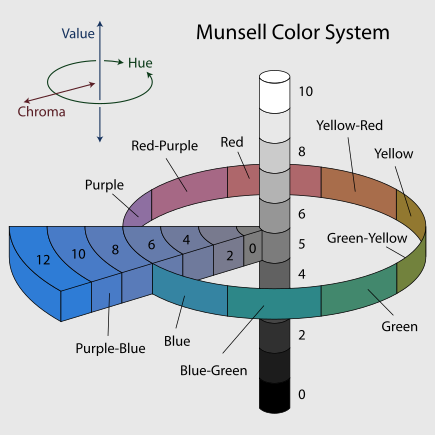
\includegraphics[width=0.4\linewidth]{source/images/munsell}
	\caption{Munsell Color System \\
		(Source: \textcite{munsell2007})}
	\label{fig:munsell}
\end{figure}
These ten hues are further subdivided a few times into ten gradations. Numbers from 0 to 10 are also added to the hues. Towards the outside, the saturation of the color (chroma) increases. The vertical center axis, which ranges from white (value 10) to black (value 0), which can be represented with colorants, is represented by the value. This results in a 10-row gray scale \parencite{munsell1915}.

\subsection{Sequential Color Scheme generator}
To develop a suitable sequential color scheme, the analytical geometry is calculated. The intersection of two subspaces is searched for. This is the intersection of the CIELAB color space and a straight line on which the color scheme lies.

For this we look which color tones lie on the straight line. This follows at given distances defined with CIEDE2000. 

It must be kept in mind that this method is only suitable for the creation of schemata that are to be used for digital maps. Therefore its construction is limited by the sRGB color space. 

This method shows a reverse approach to design color schemes based on the color distance as described in chapter \ref{subsec:equation} \parencite{brychtovaC2017}. The online tool Color Scheme Generator 1.0 has implemented this software (freely available at: http://eyetracking.upol.cz/color).

The user of this online tool can display a color scheme by selecting a base color of the whole scheme, the color classes and the CIEDE2000 color distances between the classes \parencite{brychtovaDole2015}

\section{Conclusion}

Colors that cannot be distinguished correctly and quickly are a major problem when reading choropleth maps. They can lead to errors in understanding and interpreting the map. Therefore, the choice of colors should be made carefully.

The color perception of the human eye is not stable, it is influenced by environmental light, shadows and surrounding materials. Furthermore, color perception varies from person to person and also changes over time. The extreme example is, of course, color-blind people. 

There are different color models for different purposes the RGB Color model is well known as it stand for the way color are produced ondigital screens. However other color Models try to represent colors how they are perceived by the human eye. 

It can be concluded that the ability to distinguish colors on a choropleth map is mainly influenced by the color distance. The color distance is a measure to quantify the difference between two colors or shades of a color from the perspective of the human eye. When calculating the color distance the colors need to be converted into a perceptual unitary color model it is also important to know that the color space where the selected colors are from should be sRGB to increase the chance that the colors can be created by the screens where the map is shown. 

Another aspect closely related to color spacing is the number of classes. Since colors are limited by the sRGB color space, color spacing is likely to become smaller as more classes are chosen. 

In addition, the spatial distance between two colors also affects how accurately humans can distinguish colors. The greater the spatial distance the harder it get for humans to distinguish two colors. 

Examples of useful softwares in selecting color schemes and specific colors for choropleth maps are ColorBrewer 2.0 and Sequential Color Scheme generator. The latter is definitely a tool for map makers with prior knowledge of color spacing. 

\textcite{brychtovaC2017} found that color schemes in the popular ColorBrewer 2.0 software tend to have larger color distances for dark colors, which is an indicator that darker colors are harder to differentiate. A thesis that could also be further evaluated with the ulterior motive that the color spacing calculation takes the brightness of colors into account.



%\bibliography